\section{Binární halda}\label{sec:halda}

Uveďme motivační příklad na úvod. Mějme seznam čísel, z něhož chceme (pokud možno co nejrychleji) vybrat minimální/maximální hodnotu. Pro maximum bychom sestavit následující jednoduchý algoritmus.
\begin{pseudo}{Max}[Seznam čísel $x_1,x_2,\dots,x_n$][Maximální hodnota seznamu \textit{m}]
    $m\gets x_1$\\
    \begin{For}{$i=1,2,\dots,n$}
        \begin{If}{$x_i>m$}
            $m\gets x_i$
        \end{If}
    \end{For}
\end{pseudo}

Časová složitost bude zjevně $\bigO{n}$, neboť algoritmus prochází všech $n$ prvků. Takovou úlohu lze však řešit rychleji, pokud si prvky vhodně uspořádáme. K tomu můžeme použít tzv. \emph{haldu}. 
\begin{definition}[Minimová binární halda]\label{def:binarni_halda}
    Minimová binární halda je datová struktura tvaru binárního stromu, kde v každém vrcholu je uložena \emph{právě jedna} hodnota (tzv. \emph{klíč}, pro vrchol $v$ budeme značit jeho klíč $k(v)$) a navíc platí:
    \begin{enumerate}[label=(\roman*)]
        \item\label{binhalda_podminka_1} každá hladina je \emph{plně obsazena}, kromě poslední, pričemž hladiny jsou zaplněny \emph{zleva}
        \item\label{binhalda_podminka_2} a je-li $v$ libovolný vrchol a $s$ jeho syn, pak $k(v)\leqslant k(s)$.
    \end{enumerate}
\end{definition}

\begin{figure}[h]
    \centering
    \begin{subfigure}{6cm}
        \centering
        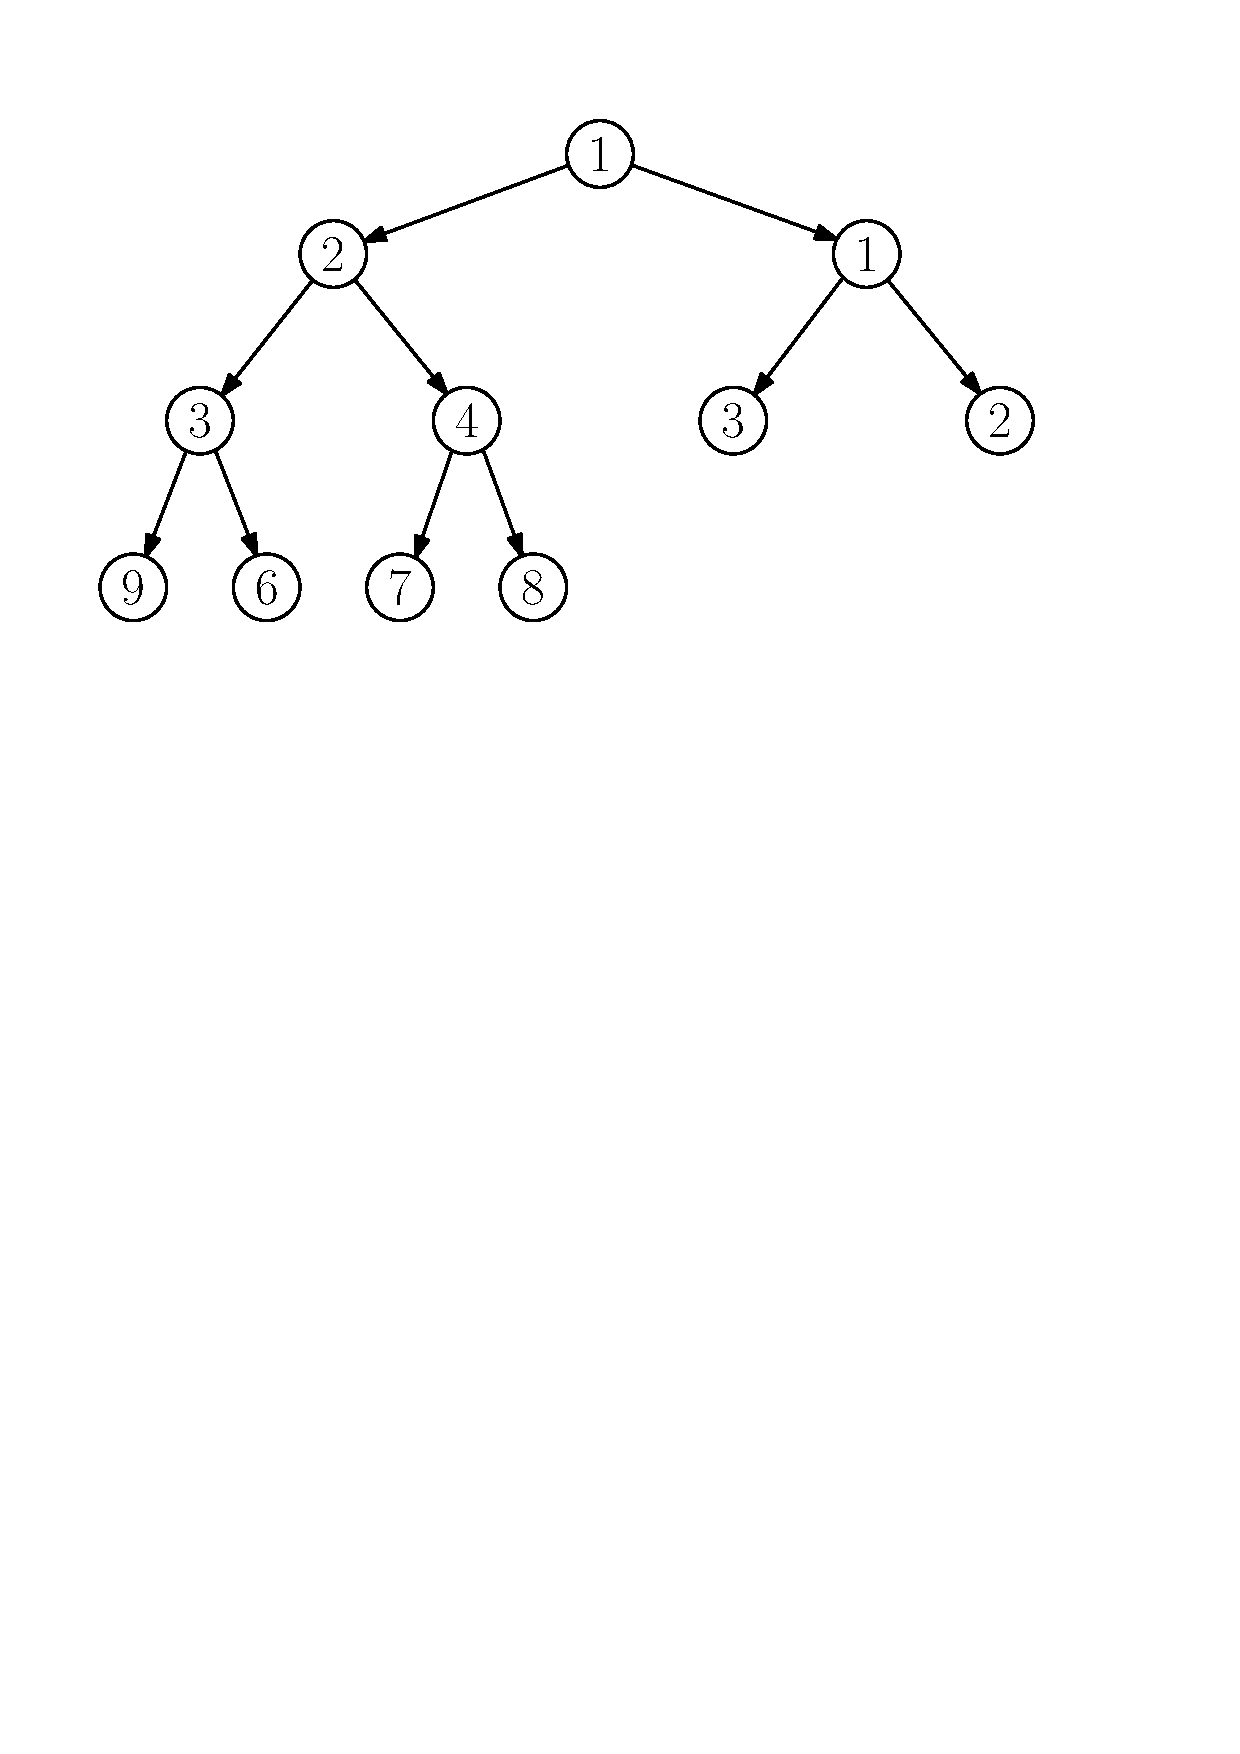
\includegraphics[scale=.4]{ch01_halda}
        \caption{Korektní halda.}
        \label{subfig:korektni_halda}
    \end{subfigure}
    \quad
    \begin{subfigure}{5cm}
        \centering
        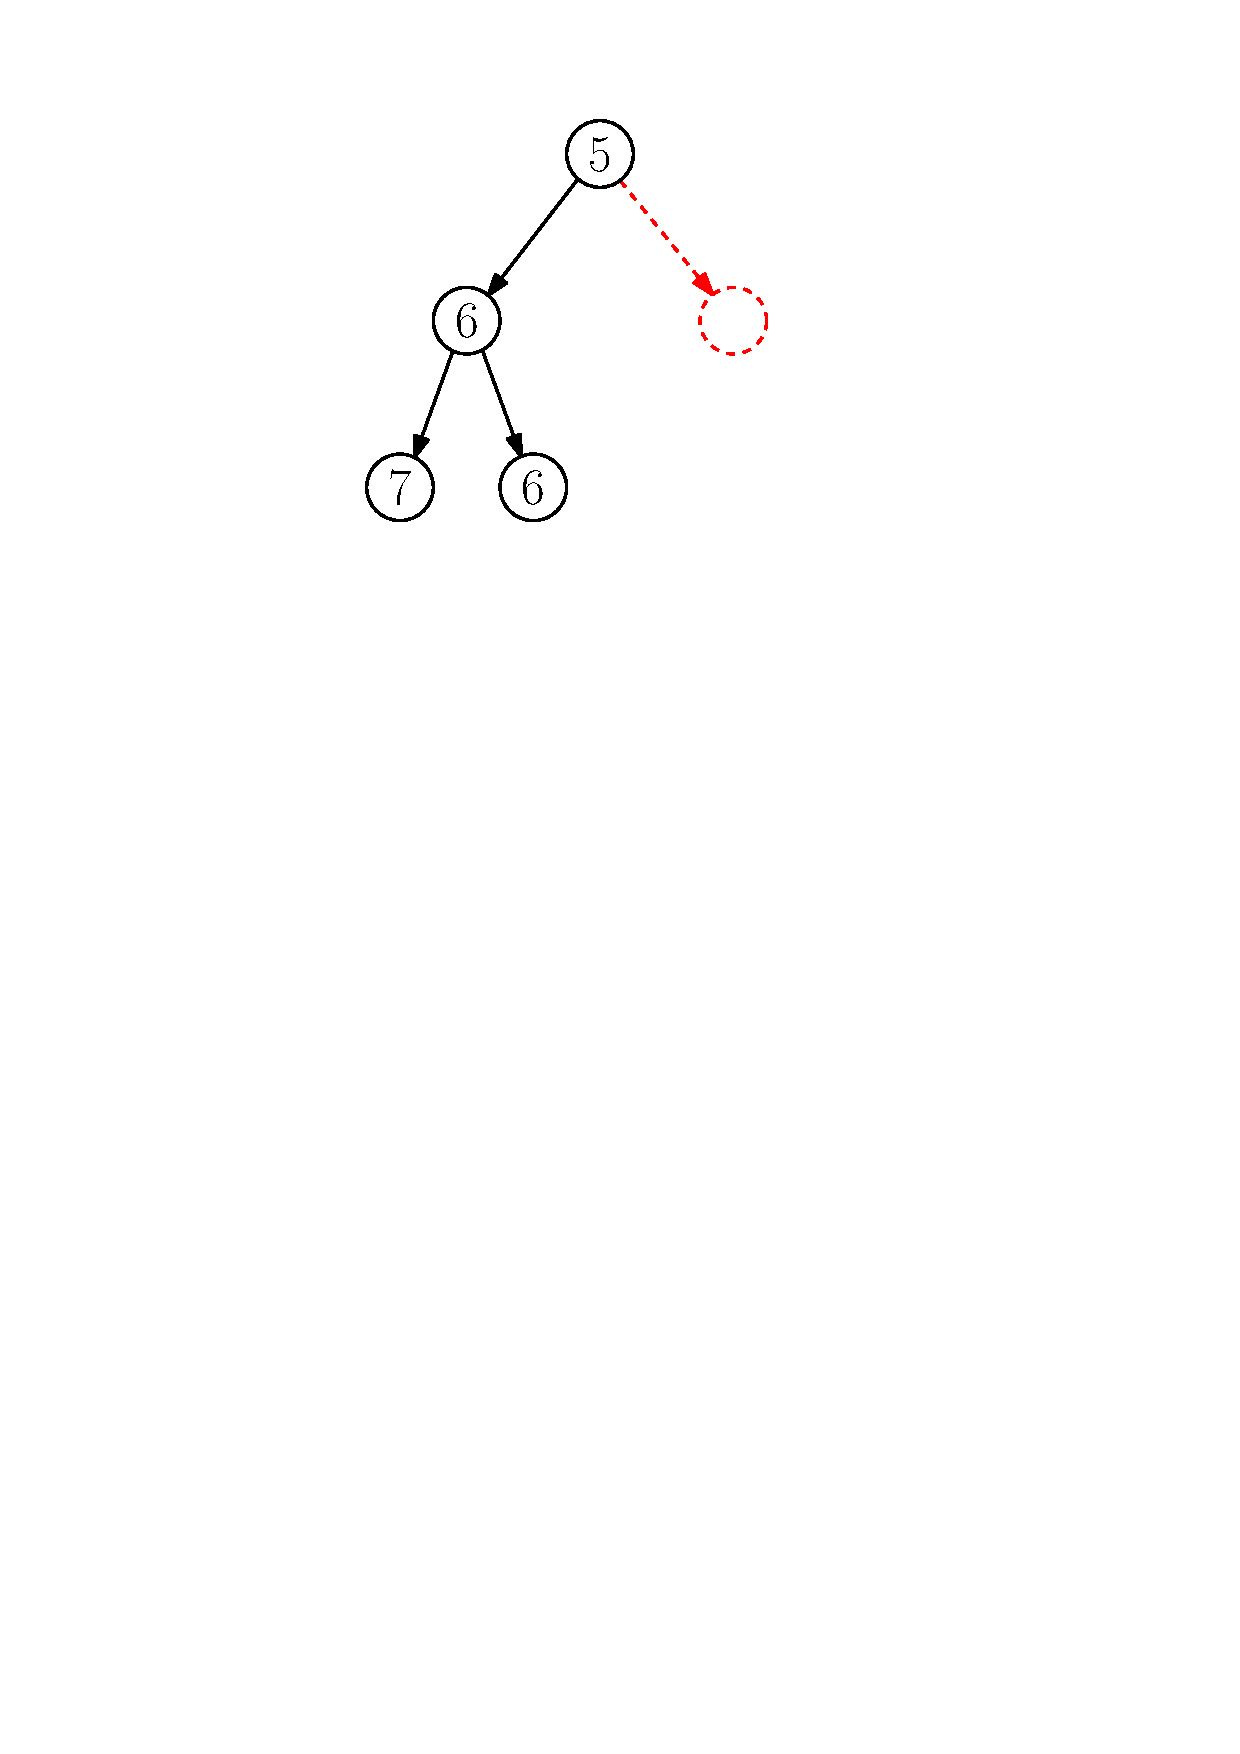
\includegraphics[scale=.4]{ch01_nekor_halda_1}
        \caption{Chybějící vrchol v 1. hladině.}
        \label{subfig:nekorektni_halda_1}
    \end{subfigure}
    \quad
    \begin{subfigure}{5cm}
        \centering
        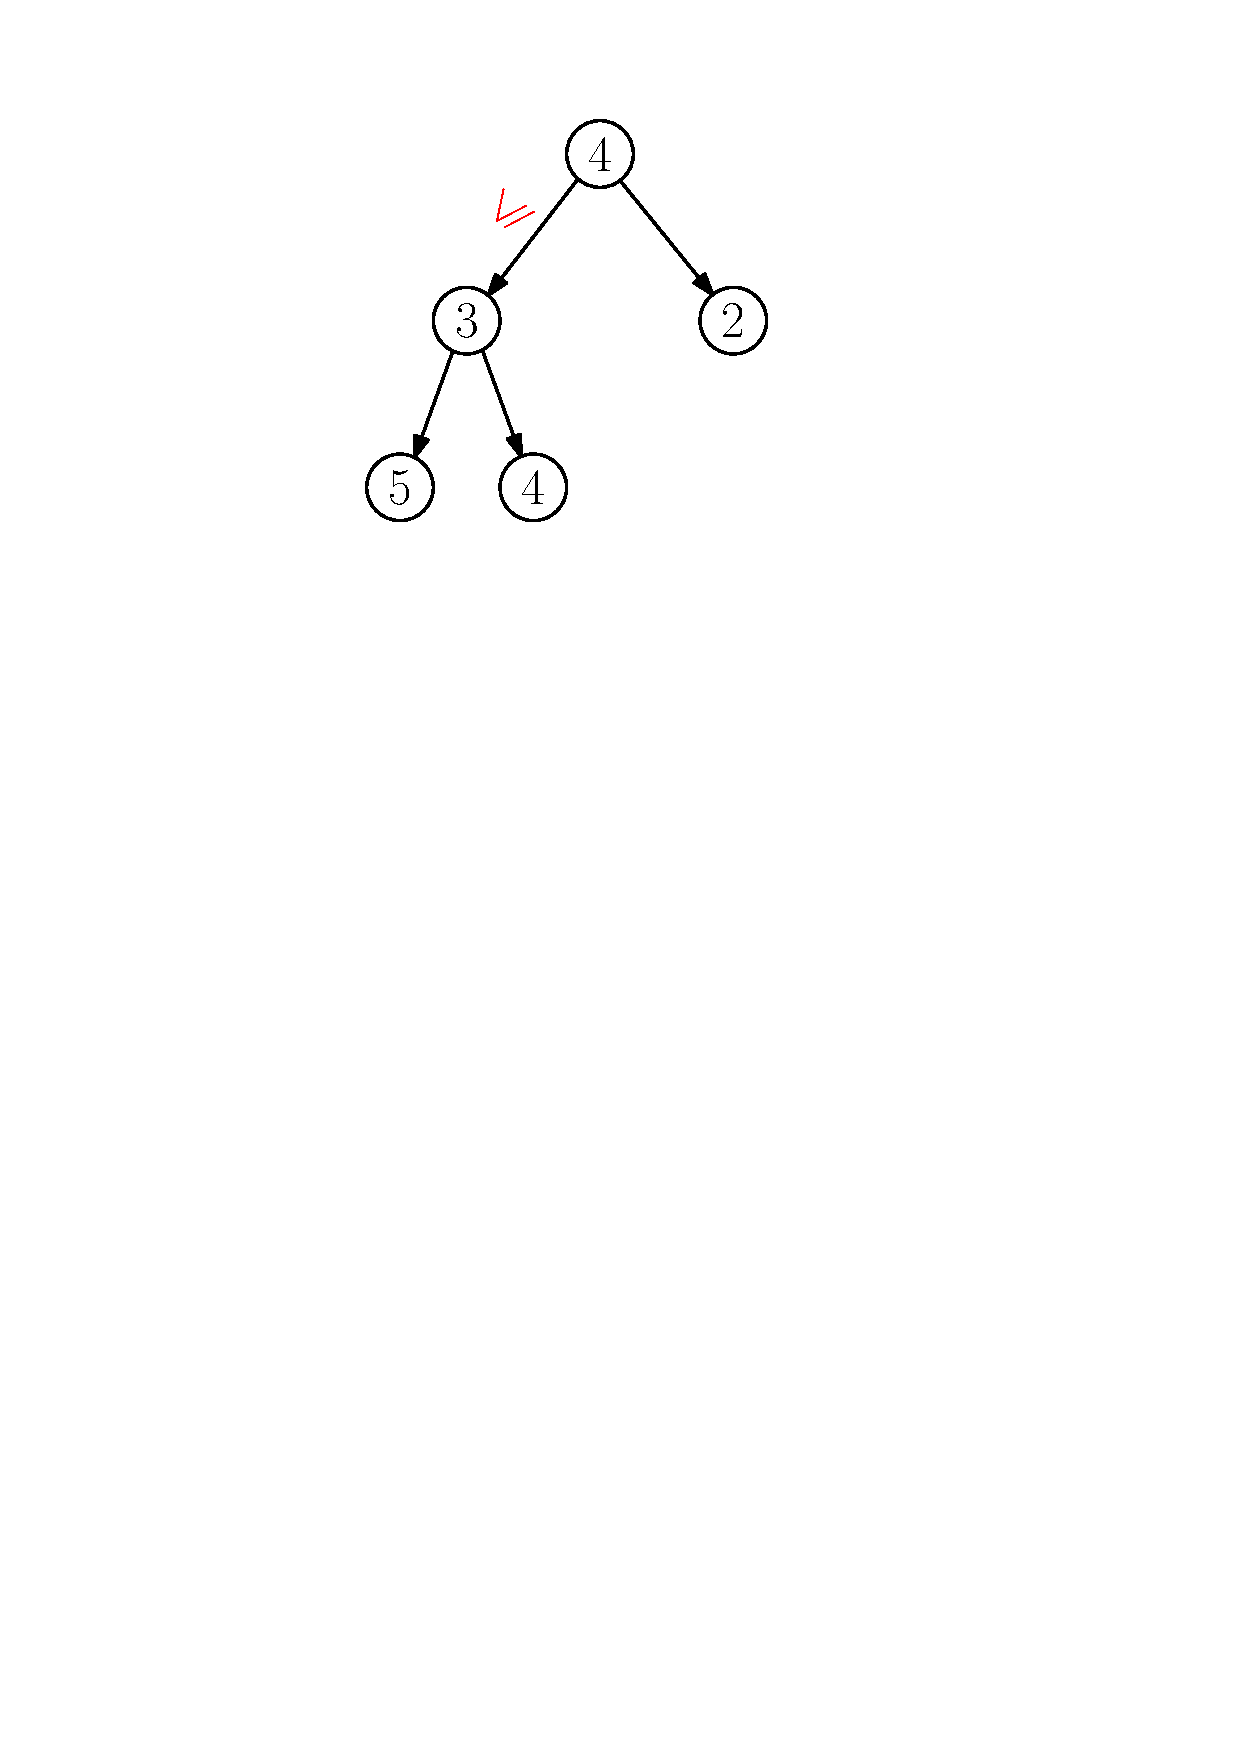
\includegraphics[scale=.4]{ch01_nekor_halda_2}
        \caption{Klíč levého syna je menší než klíč kořene.}
        \label{subfig:nekorektni_halda_2}
    \end{subfigure}
    \caption{Příklady korektních a nekorektních hald.}
    \label{fig:halda_modely}
\end{figure}

Zde se nyní na chvíli pozastavme. Podmínka \ref{binhalda_podminka_2} v definici binární haldy \ref{def:binarni_halda} má za následek totiž velmi příjemnou vlastnost, když se podíváme, kde se v haldě nachází minimum. Pokud se budeme pohybovat od kořene směrem "dolů", hodnoty ve vrcholech se budou pouze zvětšovat, neboť klíče synů mají musí mít vždy stejnou nebo větší hodnotu než klíč v rodiči. Minimum se tak vždy nachází \emph{v kořeni stromu}, což znamená, že zjistění minima tak můžeme provést v \emph{konstantním čase} $\bigO{1}$.
\notebox{Pokud bychom chtěli naopak \emph{maximovou binární haldu}, bude definice \ref{def:binarni_halda} vypadat obdobně, akorát v podmínce \ref{binhalda_podminka_2} bude obrácená nerovnost, tj. $k(v)\geqslant k(s)$ (klíč v rodiči má vždy stejnou nebo vyšší hodnotu než klíče v jeho synech). Maximum se bude opět nacházet v kořeni haldy.}
Je však více operací, které bychom rádi s haldou prováděli. Vypišme si všechny, které nás budou zajímat.
\begin{itemize}
    \item \textsc{Insert}($x$) -- \emph{vložení} nového vrcholu s klíčem $x$ do haldy.
    \item \textsc{Min}() -- \emph{nalezení} vrcholu s nejmenším klíčem (už jsme zmínili).
    \item \textsc{ExtractMin}() -- \emph{odebrání} vrcholu s nejmenším klíčem.
    \item \textsc{Increase}($v$) -- \emph{zvýšení} hodnoty klíče ve zvoleném vrcholu $v$.
    \item \textsc{Decrease}($v$) -- \emph{snížení} hodnoty klíče ve zvoleném vrcholu $v$.
\end{itemize}

Podívejme se postupně na jednotlivé operace a jejich realizaci. S dovolením si zde nyní odpustíme zápis pomocí pseudokódu a pro jednoduchost si dané operace pouze slovně vysvětlíme. Pro následné odvození časové složitosti nám to bude stačit.

\subsubsection{Vkládání nového vrcholu}

Při vkládání nového vrcholu (\textsc{Insert}) se nejdříve potřebujeme vypořádat s tím, kam vrchol v haldě umístíme. S tím nám ale pomůže podmínka \ref{binhalda_podminka_1} v definici binární haldy. Všechny hladiny stromu jsou vždy plně obsazené, kromě poslední, která se všechny vrcholy nachází vlevo. To znamená, že nový vrchol můžeme umístit na první volnou pozici vlevo na poslední hladině. To však nemůžeme provést zcela beztrestně, neboť nemáme nijak zaručeno, že bude splněna podmínka \ref{binhalda_podminka_2}. Klíč v novém vrcholu může mít hodnotu \emph{ostře menší} než jeho rodič. Haldu "opravíme" postupným prohazováním vrcholu s jeho rodičem, dokud nebude podmínka splněna (viz obrázek \ref{fig:vkladani_vrcholu_halda}).
\begin{figure}[h]
    \centering
    \begin{subfigure}{7cm}
        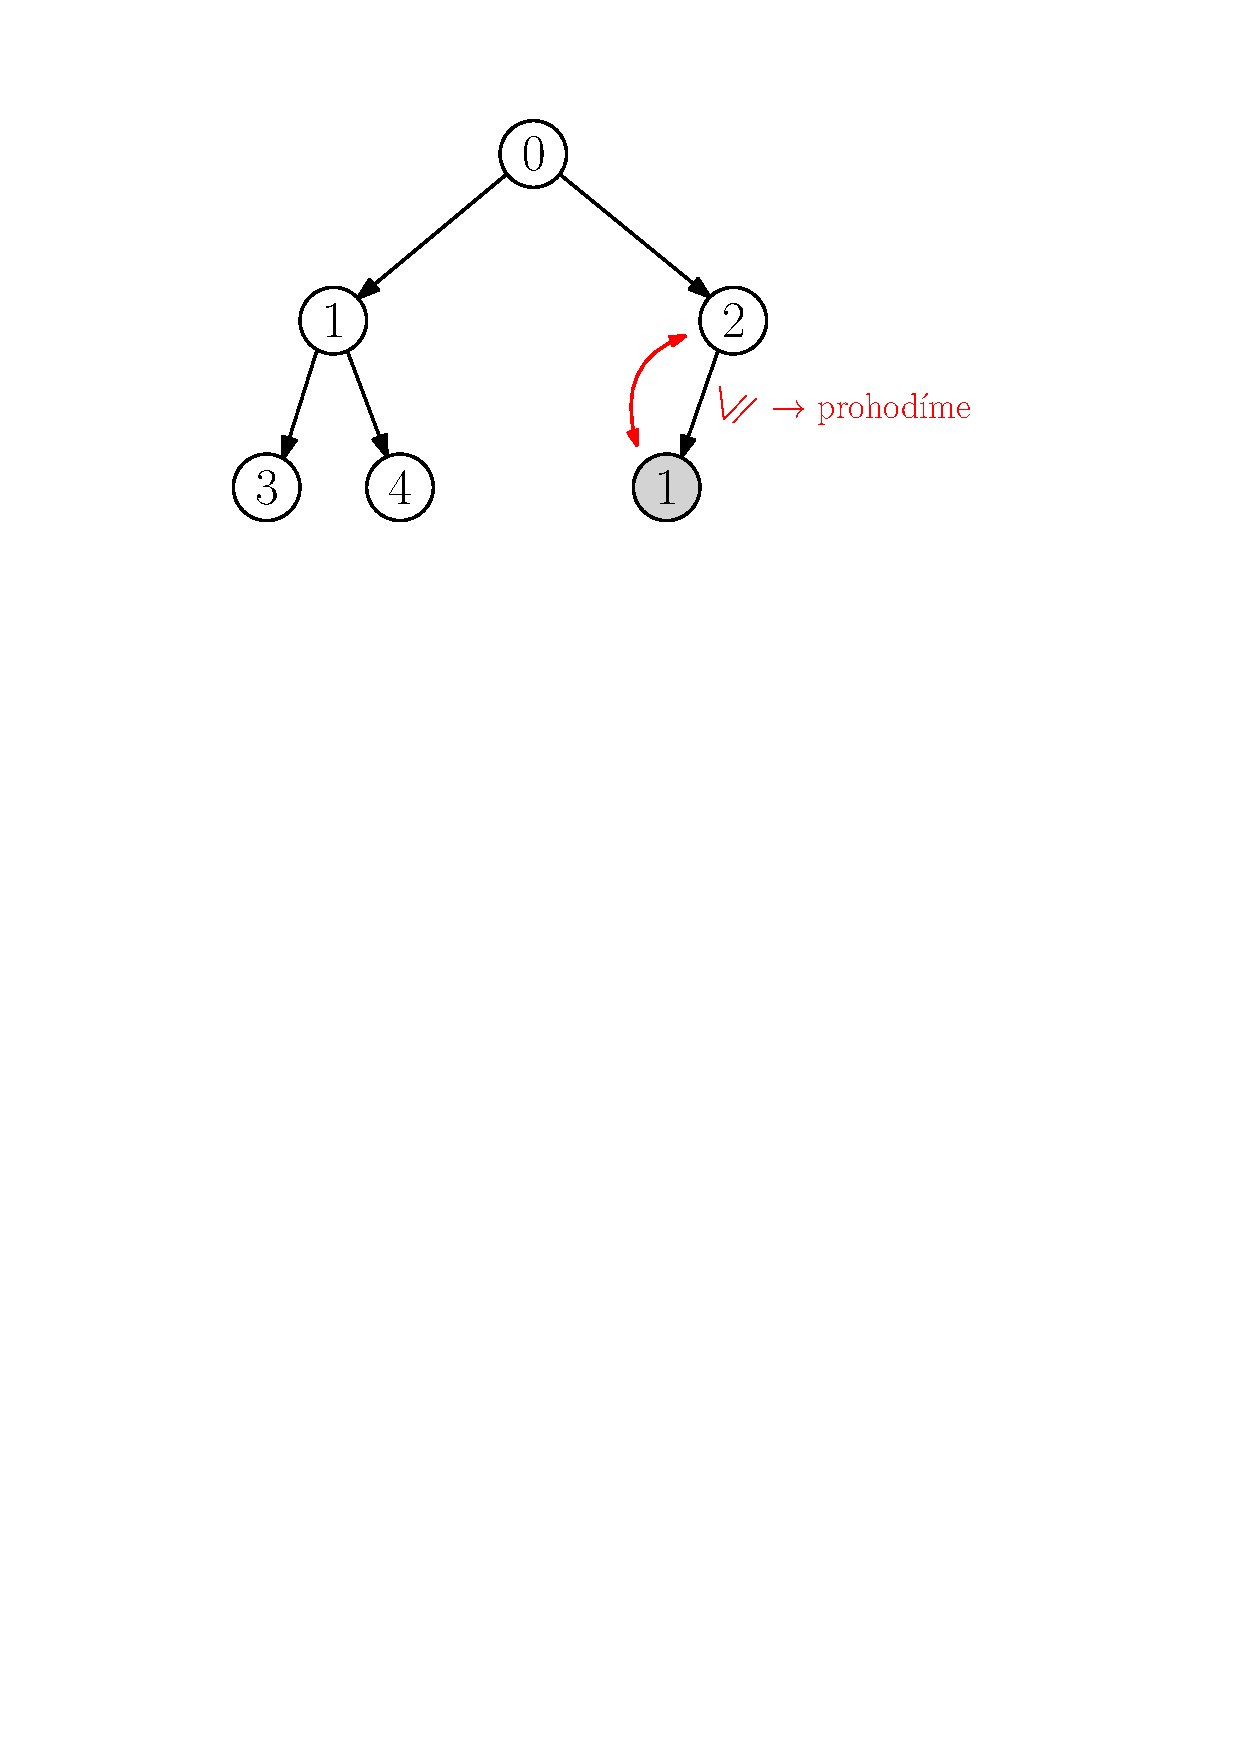
\includegraphics[scale=.5]{ch01_vkladani_1}
    \end{subfigure}
    \begin{subfigure}{7cm}
        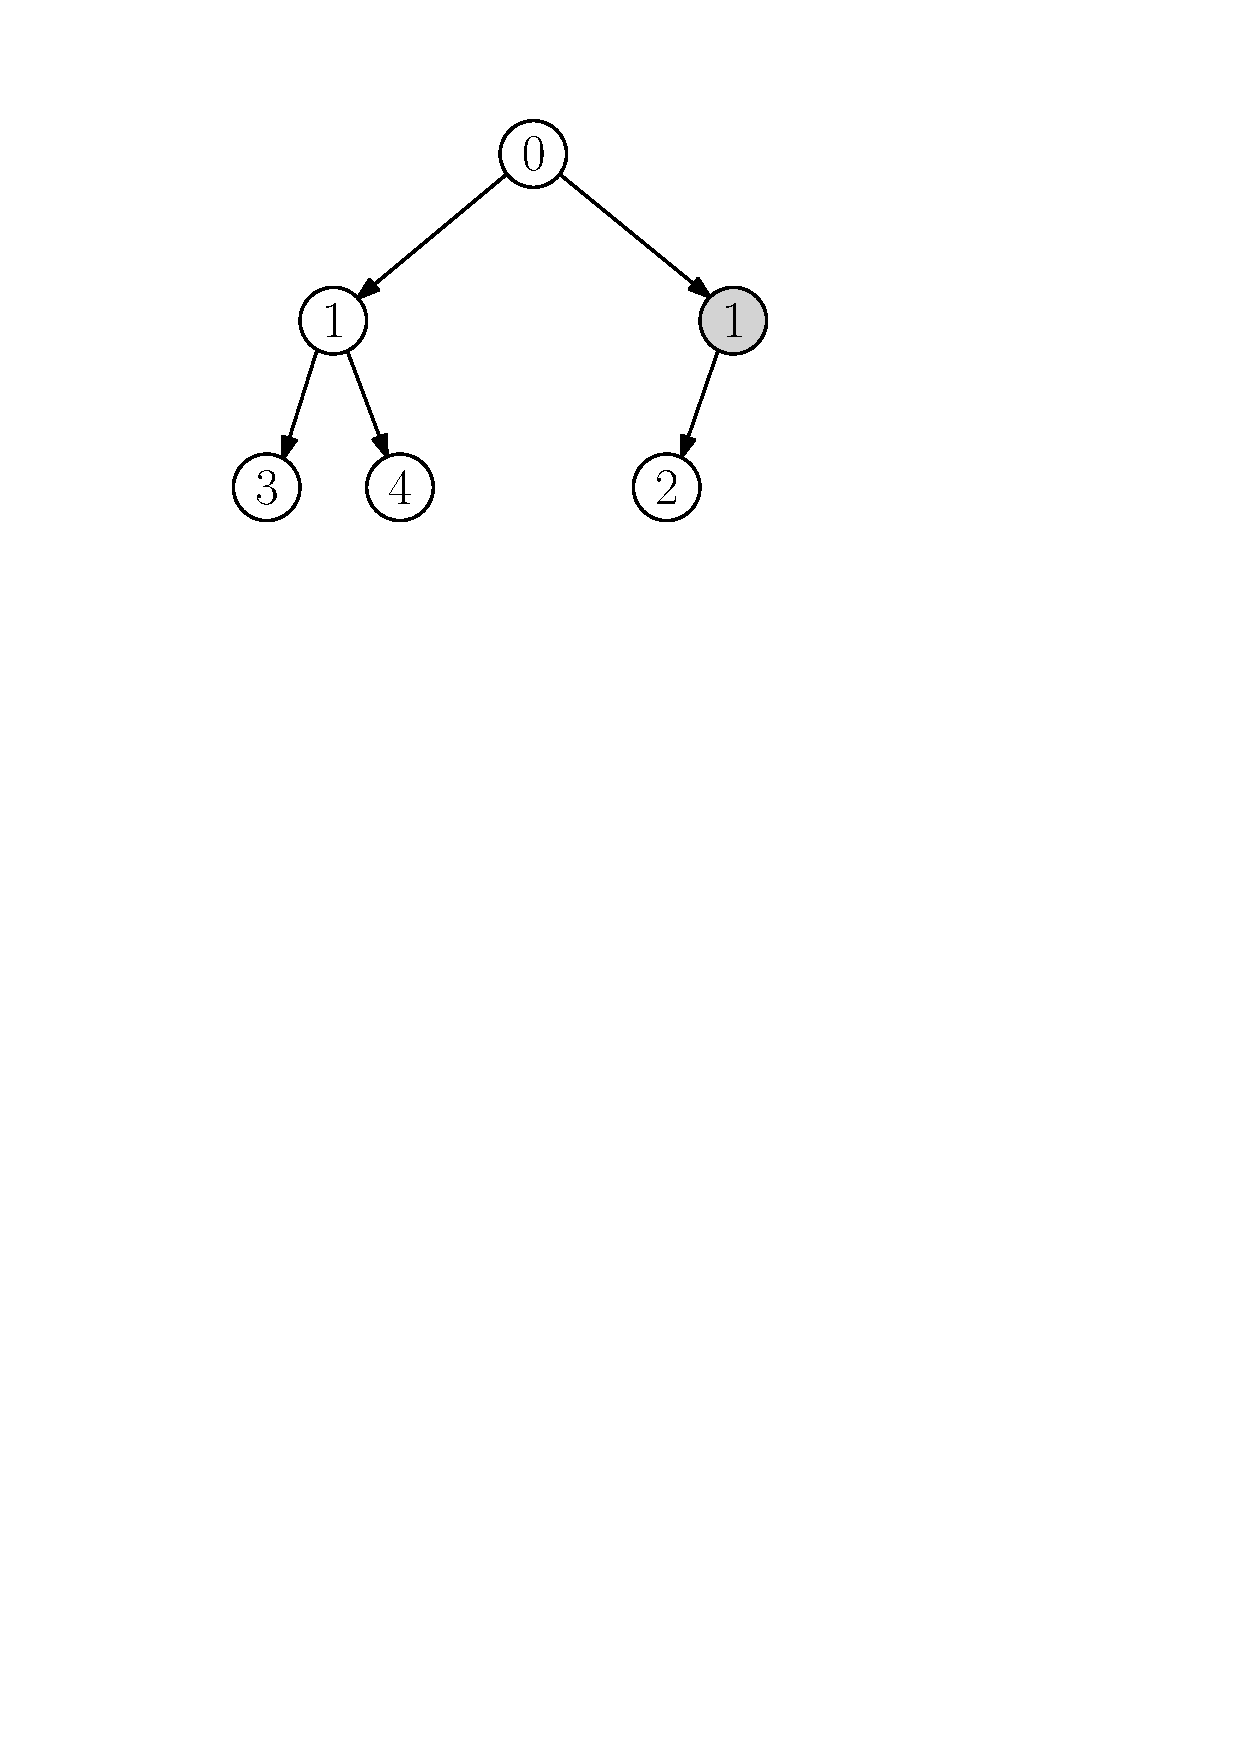
\includegraphics[scale=.5]{ch01_vkladani_2}
    \end{subfigure}
    \caption{Vkládání nového vrcholu do haldy.}
    \label{fig:vkladani_vrcholu_halda}
\end{figure}
Postup můžeme zapsat zkráceně ve dvou bodech takto:
\begin{itemize}
    \item Vložíme nový vrchol s klíčem $x$ na první volnou pozici zleva na poslední hladině.
    \item pokud je klíč rodiče větší než $x$, prohodíme vrcholy (resp. jejich klíče)\footnote{Vrchol v podstatě takto "probublá" do správné pozice ve stromě.}.
    \item Opakujeme druhý krok.
\end{itemize}